% !TEX root = ../main.tex

\chapter{词嵌入模型}

近些年,作为机器学习最重要的一个分支,深度学习成为科研人员关注的热点问题,并且深度学习模型在计算机视觉、自然语言处理、语音识别、数据挖掘等领域发挥了至关重要的作用。深度学习模型通过使机器模仿人类的感官和思想方式,挖掘大量的、多维度数据背后的潜在规则,解决了很多复杂的模式识别疑难问题,为人类迈向人工智能做出了突出贡献。不仅仅在上述领域,如今在生物信息学和基因组学方面,深度学习也带来了巨大的改变。在大数据时代,深度学习通过将生物医学大数据转化为有价值的领域知识极大简化了蛋白质功能研究和药物发现研究的历程。

传统的机器学习方法在研究的过程中,科研人员需要利用特征工程手动在原始序列数据的领域知识上提取特征,然后再部署相关的机器学习算法,这样的做法比较耗时而且极大的依赖于生物信息学和基因组学的专业知识。随着深度神经网络的兴起,传统的特征提取方法已经在很大程度上被序列编码方法,即词嵌入表征学习所取代。深度学习模型通过将组成生物序列的单词编码成稠密、连续的低维向量获得比离散特征提取表示更好的性能。由于在 NLP 领域的词向量和深度学习技术已经趋于成熟,同时生物序列和文本序列具有一定的相似性,可以通过将 NLP 中的词嵌入方法和深度学习模型迁移到生物信息学进行深入研究和探索。本章将重点介绍 NLP 领域中的词嵌入方法。

词嵌入是文本的学习表示,其中单个词在预定义的向量空间中表示为实值向量,这种表示单词和文档的方法被认为是深度学习在自然语言处理问题上的关键突破之一。将每个词都映射到一个向量,向量中的值以类似于神经网络的方式学习,因此该技术通常被归入深度学习领域。该方法的关键是对每个单词表示为密集分布式,即每个词都由一个实值向量表示,通常是数十或者数百维,这与稀疏词表示(例如 one-hot 编码)所需的数千或数百万维度形成对比。词汇表中的每个单词关联到一个分布式单词的特征向量,特征向量代表词的不同方面,每个单词与向量空间中的一个点相关联,其中特征的数量远小于词汇量。分布式表示是基于单词的使用来学习的,这允许以相似方式使用的单词产生相似的表示,自然地捕捉它们的含义,这与词袋模型中清晰但是忽略单词上下文顺序的表示形成对比。使用密集、低维向量的好处之一是:大多数神经网络工具包不能很好地处理非常高维的稀疏向量;另一个主要好处是良好的泛化能力,如果我们相信某些特征可能提供类似的线索,那么能够捕捉这些相似性的表示是值得的,即具有相似上下文的单词将具有相似的含义。

\section{基于离散表示的词嵌入方法}
\subsection{one-hot 编码}
我们可以用数字表示单词的最基本方法之一是通过 one-hot 编码(独热编码)方法。这个想法超级简单,创建一个向量,其维度与语料库中的出现的单词数量一样多。将每一个单词表示为 $\mathbb{R}^{|V|\times1}$ 向量,其中 $|V|$ 表示词汇量的大小,每个唯一的单词都有一个唯一的维度,并且将在该维度中用 1 表示,其他地方都是 0。这种类型的编码词向量示例如公式 (\ref{equ:3-1})所示:

\begin{equation}
    \omega^{aardvark} = \begin{bmatrix}1\\0\\0\\\vdots&\\0\\ \end{bmatrix}, \omega^{a} = \begin{bmatrix} 0 \\ 1 \\ 0 \\ \vdots& \\ 0 \\\end{bmatrix}, \omega ^{at} = \begin{bmatrix} 0 \\ 0 \\ 1 \\ \vdots& \\ 0 \\\end{bmatrix}, \dots, \omega ^{zebra} = \begin{bmatrix} 0 \\ 0 \\ 0 \\ \vdots& \\ 1 \\\end{bmatrix}.
\label{equ:3-1}
\end{equation}

通过 one-hot 编码得到的词嵌入表征向量是巨大而稀疏的向量,每个单词被表示为一个完全独立的实体,完全没有捕获任何相似关系的信息完全忽略了语义关系信息,例如公式(\ref{equ:3-2})所示。

\begin{equation}
    (\omega^{hotel})^{T}\omega^{motel} = (\omega^{hotel})^{T}\omega^{cat} = 0.
\label{equ:3-2}
\end{equation}

所以也许我们可以尝试从将这个空间的大小从 $\mathbb{R}^{|V|}$ 减小到某个值,从而找到一个编码单词之间关系的子空间。

\subsection{TF-IDF 编码}
TF-IDF 算法是一种基于加权算法的统计词频技术,常常用于信息检索和数据挖掘领域。TF-IDF 算法包含两部分:一部分是 TF(Term Frequency),即词频;另一部分是 IDF(Inverse Document Frequency),即逆文档频率。

经常出现但无处不在的词语应该被赋予很少的权重或意义,这类词称为停用词,例如英语中的 or 和 and,它们不能提供很大的价值。通过计算 TF 可以统计这些停用词,设置单词出现的频率,将它们过滤掉。如果一个词很少出现或经常出现,但只出现在一个或两个地方,那么这些词可能是更重要的词,因此应该进行加权。IDF 的指标与 TF 正好相反,它通常给常见的单词赋予较小的权重,即 IDF 的值与单词在所有文本中的常见程度成反比。

TF-IDF 算法的流程如下所示:
\begin{itemize}
    \item 第一步:计算 TF(词频);
    \begin{equation}
        TF\mbox{(词频)}= \mbox{某个词在文章中的出现次数}.
    \end{equation}
    \item 由于每篇文章的长短不同,通过将 TF 标准化使得不同长度的文章可以进行比较;
    \begin{equation}
        TF\mbox{(词频)}= frac{\mbox{某个词在文章中的出现次数}}{\mbox{文章的总次数}}.
    \end{equation}
    \item 第二步:计算 IDF(逆文档频率);
    \begin{equation}
        IDF\mbox{(逆文档频率)} = log(frac{\mbox{语料库的文档总数}}{\mbox{包含该词的文档数}+1}). 
    \end{equation}
    从上式可见,如果一个单词在语料库中出现的越频繁,分母就越大,IDF(逆文档频率)就越接近于 0 ;
    \item 第三步:计算 TF-IDF;
    \begin{equation}
        TF-IDF = TF\mbox{(词频)} \times IDF\mbox{(逆文档频率)}. 
    \label{equ:3-3}
    \end{equation}
\end{itemize} 

从公式(\ref{equ:3-3})中可以看到,TF-IDF 与单词在当前文档中的词频成正比,与该单词在语料库中所有文档的词频成反比。所以,通过计算当前文档的每个单词的TF-IDF 值,由大到小降序排列,排在最前面的几个单词就是当前文档的关键词,有较高的权重。

TF-IDF 算法的好处在于计算简单,容易理解,但是缺点也很明显。通过词频判断单词在文本中的重要性较为片面,有些特殊情况关键字在文本中的出现次数并不高,同时此算法无法体现单词之间的位置顺序关系,因此最终结果可能不太准确。


\section{基于 SVD 分解的词嵌入方法}
one-hot 编码方法得到的向量长度为词汇表的大小,在动辄包含上万词汇的语料库中,这样的编码表征方法有着严重的维数灾难问题。one-hot 编码方法假设每一个单词都是相互独立的,我们可以通过提取单词之间的共性,将单词的表征维度进行压缩,在较小的特征空间中使用连续稠密的低维向量表示每一个单词不同维度的抽象特征,其中每一个向量维度代表了提取到的一个抽象特征属性。

词袋假说可以得到上述分布式的表征向量。构造一个文档矩阵 $A$,其中矩阵 $A$ 的每一行 $A_{i,:}$ 表示词汇表中的一个单词,矩阵 $A$ 的每一列 $A_{:,j}$ 表示语料库中的一篇文档。矩阵中的每一个元素 $A_{i,j}$ 表示单词 $w_i$ 在文档 $D_j$ 中的频率,可以通过深度学习训练提取矩阵中的行向量作为单词的语义表征向量,列向量作为文档的主题表征向量。

SVD 分解(奇异值分解)方法基于词袋假说,将一个较大的复杂矩阵分解为多个较小的简单矩阵相乘,每一个简单矩阵包含了复杂矩阵的重要特性。我们首先循环处理语料库中的文本并累积得到单词共现计数矩阵 $X$,然后对矩阵 $X$ 执行奇异值分解以获得 $USV^{T}$ 的矩阵相乘。我们可以使用矩阵 $U$ 的行向量作为词汇表中单词的词嵌入表征向量。

\subsection{单词-文档矩阵}
假设相关的词将经常出现在同一文档中,例如,”银行”、“债券”、“股票”、“货币”等很可能会一起出现,但是“银行”、“章鱼”、“香蕉”和“足球”等单词可能不会一直一起出现。我们使用这个假设构建一个单词-文档矩阵 $X$:循环数十亿个语料库中的文档,每当单词 $w_i$ 在文档 $D_j$ 中出现时,我们就将矩阵中的元素 $X_{ij}$ 加一。 这显然是一个非常大的矩阵 ($\mathbb{R}^{|V| \times M}$),它随着文档的数量 ($M$) 进行缩放。

\subsection{基于窗口的单词共现矩阵}
矩阵 $X$ 存储单词的共现次数,从而成为亲和矩阵。在这种方法中,我们遍历语料库中所有的单词,计算每个单词在其周围特定大小的窗口中出现的次数。例如我们的语料库只包含三个句子:
\begin{itemize}
    \item I enjoy flying.
    \item I love NLP.
    \item I like deep learning.
\end{itemize}

我们使用窗口大小为 1 得到的单词共现矩阵如下:

\begin{equation}
    X = \bordermatrix{
        & I & like &enjoy & deep & learning & NLP & flying & . \cr
    I    & 0 & 2 & 1 & 0 & 0 & 0 & 0 & 0 \cr
    like & 2 & 0 & 0 & 1 & 0 & 1 & 0 & 0 \cr
    enjoy & 1 & 0 & 0 & 0 & 0 & 0 & 1 & 0 \cr
    deep & 0 & 1 & 0 & 0 & 1 & 0 & 0 & 0 \cr
    learning & 0 & 0 & 0 & 1 & 0 & 0 & 0 & 1 \cr
    NLP & 0 & 0 & 1 & 0 & 0 & 0 & 0 & 1 \cr
    flying & 0 & 0 & 1 & 0 & 0 & 0 & 0 & 1 \cr
    . & 0 & 0 & 0 & 0 & 1 & 1 & 1 & 0 \cr
    },
\end{equation}

\subsection{将 SVD 分解应用于单词共现矩阵}
我们对矩阵 $X$ 执行 SVD 分解(如公式(\ref{equ:SVD-1})所示),观察奇异值(结果矩阵 $S$ 中的对角线项),并且根据所需的百分比方差在某个索引 $k$ 处将它们截断,选择前 $k$ 个奇异向量来降低维度:

\begin{equation}
    frac{\sum_{i=1}^{k}\sigma_i}{\sum_{i=1}^{|V|}\sigma_i}
\end{equation}

然后我们将 $U_{1:|V|,1:k}$ 的子矩阵作为我们的词嵌入表征矩阵,他们提供了词汇表中每个单词的 $k$ 维表示向量(如公式(\ref{equ:SVD-2})所示)。

\begin{equation}
    \resizebox{.9\hsize}{!}{X = \bordermatrix{
        &  & |V| &   \cr
        &  &  &      \cr
    |V| &  & X &     \cr
        &  &  &      \cr
    } = |V| \bordermatrix{
        &  & |V| &   \cr
        & | & | &   \cr
        & u_1 & u_2 & \cdots \cr
        & | & | &   \cr
    } |V| \bordermatrix{
        &  & |V| &   \cr
        & \sigma_1  & 0 & \cdots  \cr
        & 0 & \sigma_2 & \cdots \cr
        & \vdots & \vdots & \ddots  \cr
    } |V| \bordermatrix{
        &  & |V| &   \cr
        & - & v_1 & -   \cr
        & - & v_2 & - \cr
        &  & \vdots &   \cr
    }},
\label{equ:SVD-1}
\end{equation}

\begin{equation}
    \resizebox{.85\hsize}{!}{X = \bordermatrix{
        &  & |V| &   \cr
        &  &  &      \cr
    |V| &  & \hat{X} &  \cr
        &  &  &      \cr
    } = |V| \bordermatrix{
        &  & k &   \cr
        & | & | &   \cr
        & u_1 & u_2 & \cdots \cr
        & | & | &   \cr
    } k \bordermatrix{
        &  & k &   \cr
        & \sigma_1  & 0 & \cdots  \cr
        & 0 & \sigma_2 & \cdots \cr
        & \vdots & \vdots & \ddots  \cr
    } k \bordermatrix{
        &  & |V| &   \cr
        & - &v_1& -   \cr
        & - &v_2& - \cr
        &  & \vdots &   \cr
    }},
\label{equ:SVD-2}
\end{equation}

基于 SVD 奇异值分解得到的词嵌入表征向量为我们提供了足以编码语义和句法(词性)信息的词向量,但是仍然存在一些问题。比如: SVD 分解方法不适用于大矩阵,因为复杂矩阵进行奇异值分解的训练成本较高;由于大多数单词不会同时出现,所以得到的单词共现矩阵非常稀疏;当有新词或者新文档的加入时,矩阵的维度变化非常大。下面将介绍基于神经网络的词嵌入方法,可以解决以上的问题。

\section{基于神经网络的词嵌入方法}
词嵌入(Word Embedding)是一种将文本中的单词转化为稠密数字向量的方法。为了使计算机能够识别输入的特征,就需要把这些被转换成数字的向量以数字形式作为输入使用深度学习模型进行分析。

早期的词嵌入方法通常采用独热编码(One-hot)的方式,它使用一个词汇表大小的向量来表示文本中的词,其中只有对应于该词的项是1而所有其他的项都是零。One-hot 编码的最大问题在于不能表示词与词之间的相似性。我们通过点积计算向量之间的相似性。在One-hot编码中,语料库中任何两个词之间的点积总是为零,即任意两个词是正交的。随着深度学习的兴起,基于深度学习的词嵌入方法能够在没有任何人的干预下自主学习单词的潜在语义,同时可以表示词与词之间的相似性。我们不需要计算和存储关于某个庞大的数据集(可能是数十亿个句子)的全局信息,我们可以尝试创建一个模型,该模型将能够一次学习一个迭代,并最终能够根据上下文对单词的概率进行编码。其思想是设计一个以词向量为参数的模型。然后,针对特定的目标函数对模型进行训练。在每次迭代中,我们运行通过运行模型计算误差,并遵循相应的参数更新规则,该规则可以对导致误差的错误进行惩罚。通过这种机制,我们学习到了模型的词嵌入表征。目前,基于深度学习的词嵌入方法已经广泛应用于 NLP 领域的各种任务中,例如文本分类,情感分析,机器翻译等等。

蛋白质序列同自然语言处理中的文本一样,由很多单词排列组合构成。蛋白质序列由20几种连续的氨基酸构成,是研究蛋白质功能的基础。我们可以将组成蛋白质序列的氨基酸类比于组成文本的单词,将蛋白质序列信息类比于文本中句子的语义信息。因此,NLP 领域中的词嵌入方法非常适合于蛋白质序列领域的研究,下面将介绍4种本文用到的词嵌入方法。

\subsection{Word2Vec}
Word2Vec \cite{mikolov2013distributed} 词嵌入表征是由 Mikolov 等人于 2013 年提出的一种词嵌入方法。它包含两个学习模型,分别是 continuous bag-of-words (CBOW) 和 skip-gram. CBOW 旨在根据词向量从上下文信息中预测中心词,skip-gram则做了相反的事情,它从中心词预测上下文单词的分布(概率)。

\begin{figure}[!htp]
\centering
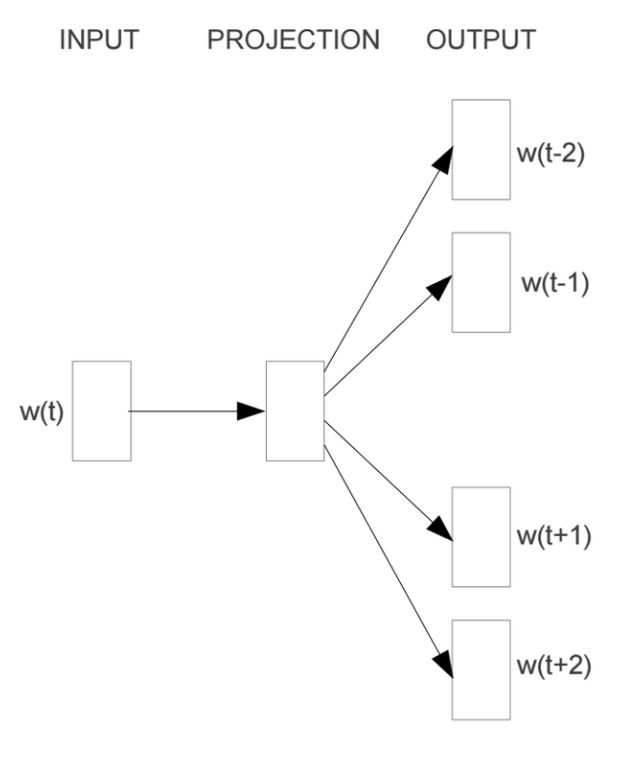
\includegraphics[width=0.6\textwidth]  {imgs/skip-gram.png} \\
\bicaption[Skip-gram\cite{mikolov2013distributed}图示]
    {Skip-gram\cite{mikolov2013distributed}图示。}
    {Model architecure of Skip-gram\cite{mikolov2013distributed}.}
\label{fig:skip-gram}
\end{figure}

这里我们以 skip-gram 模型为例详细的介绍。如图 \ref{fig:skip-gram} 所示,我们假设上下文的窗口为$2m$,即以中心词为中心,分别向左和向右选取$m$个单词,那么给定中心词预测上下文单词的概率为:

\begin{equation}
    P(\omega_c|\omega_o) = \frac{exp(u_o^{T} v_c)}{\sum_{i \in V} exp(u_i^{T} v_c)},
\end{equation}
其中 $\omega_o$ 和 $\omega_c$ 分别代表中心词和上下文单词,$u_o$和$u_c$分别代表中心词向量和上下文词向量,$V$是全体词汇表。这个概率就是给定中心词的条件下,某个词是上下文词的概率。这里假设在给定中心词的条件下每个单词出现的概率是独立的,类似朴素贝叶斯的条件独立性假设,可以大大的简化运算,将上式改写为连乘的形式如下:

\begin{equation}
   \prod \limits_{t=1}^T \prod \limits_{-m\leq j \leq m, j \neq 0} P(\omega^{(t+j)}|\omega^{(t)}),
\end{equation}
其中$t$表示中心词的位置,$m$为窗口大小,这样就得到了每个中心词的计算上下文词的概率。在该公式中变量是上下文词向量和中心词向量,于是只要改变参数使得目标最大化就可以。这里使用极大似然估计,对上式取负对数得到:

\begin{equation}
   -\sum \limits_{t=1}^T \sum \limits_{-m\leq j \leq m, j \neq 0} log^{P(\omega^{(t+j)}|\omega^{(t)})}.
\end{equation}

对上式进行参数求导可以计算梯度,更新参数。梯度下降优化结束后,我们便能得到两个向量 $u$ 和 $v$,分别表示上下文词向量和中心词向量,这就是我们要找的词向量。

Word2Vec作为预训练的词嵌入方法,通常语料库包含上千万条数据,词汇表中的单词数量通常有上万个,因此在目标函数中计算所有单词的softmax概率需要消耗巨大的计算资源。对此,Mikolov等人提出了负采样和层级softmax方法简化模型的复杂度和参数量。

负采样的思想为,对于每个训练步骤,我们可以只采样几个反例而不是计算整个词汇表。层级 softmax 使用二叉树来表示词汇表中的所有单词。二叉树的每一个叶子节点都表示一个单词,从根节点到叶子节点都有一条独特的路径。一个单词作为输出词的概率表示为从根节点随机游走到该词叶节点的概率。计算成本从 $O(V)$ 降低为 $O(log^{V})$。

Daniel 和 David 等人 \cite{buchan2019inferring} 使用 Word2Vec 证明了蛋白质域在多域蛋白质的上下文中可能具有语义意义。在这项工作中,他们将多域蛋白质视为文本中的句子,其中域标识符视为句子中划分的单词。 通过使用 Interpro \cite{finn2017interpro} 真核蛋白质作为语料库,他们证明了 Word2Vec 可以获得具有功能意义的蛋白质域嵌入。


\subsection{GloVe}
Word2Vec 模型通过在上下文窗口中进行预测来学习单词嵌入,该模型具有捕获单词相似性的复杂语言模式的能力,但是未能利用全局共现统计。GloVe \cite{pennington2014glove} 是由 Pennington 等人于2014年提出的基于单词共现统计的词嵌入方法。相比之下,GloVe 由一个加权最小二乘模型组成,该模型在全局单词-单词间共现概率矩阵上进行训练,从而有效地利用了统计数据。 该模型生成了一个具有有意义子结构的词向量空间。它在单词类比任务上显示了最先进的性能,并且在几个单词相似性任务上优于其他的方法。

首先定义词与词之间的共现矩阵为 $X$,其中 $X_{ij}$ 是语料库中出现在单词 $i$ 上下文中单词 $j$ 的次数。定义 $X_i = \sum_{k} X_{ik}$ 表示单词 $i$ 的上下文所有单词的总个数。最终 $P_{ij} = P(j|i) = \frac{X_{ij}}{X_i}$ 表示单词 $j$ 出现在单词 $i$ 上下文的概率。

\begin{table}[!htbp]
\centering
\bicaption[GloVe \cite{pennington2014glove} 中共现矩阵示例]{GloVe \cite{pennington2014glove} 中共现矩阵示例。}{Example of GloVe \cite{pennington2014glove} co-occurrence matrix.}
\scalebox{1.25}{
\begin{tabular}{c|c|c|c|c}
\hline
概率和比率 & k=solid & k=gas & k=water & k=fashion\\
\hline
$P(k|ice)$ & $1.9\times10^{-4}$ & $6.6\times10^{-5}$ & $3.0\times10^{-3}$ & $1.7\times10^{-5}$\\
\hline
$P(k|stream)$ & $2.2\times10^{-5}$ & $7.8\times10^{-4}$ & $2.2\times10^{-3}$ & $1.8\times10^{-5}$\\
\hline
$P(k|ice)/p(k|stream)$ & 8.9 & $8.5\times10^{-2}$ & 1.36 & 0.96\\
\hline
\end{tabular}}
\label{tabel:glove-1}
\end{table}

表\ref{tabel:glove-1}表明,单词的词向量应该和单词共现概率的比率有关,而不是他们的概率本身。由表\ref{tabel:glove-1}看出 $P(i|k)/P(j|k)$ 的取值是有一定规律的,定义函数 $F(w_i,w_j,w_k) = P(i|k)/P(j|k)$, Pennington 等人对共现概率的比率进行了总结如表 \ref{table:glove-2} 所示:

\begin{table}[!htbp]
\centering
\bicaption[GloVe \cite{pennington2014glove} 中共现概率比率的规律。]{GloVe \cite{pennington2014glove} 中共现概率比率的规律。}{The law of GloVe \cite{pennington2014glove} co-occurrence probability ratio.}
\scalebox{1.2}{
\begin{tabular}{c|c|c}
\hline
$F(w_i,w_j,w_k)$ & 单词j,k相关 & 单词j,k不相关 \\
\hline
单词i,k相关 & 趋近于1 & 很大 \\
\hline
单词i,k不相关 & 很小 & 趋近于1\\
\hline
\end{tabular}}
\label{table:glove-2}
\end{table}

GloVe经过推理,定义目标函数(损失函数)如下:

\begin{equation}
  J = \sum \limits_{ik} f(X_{ik}){(w_i^{T}w_k + b_i + b_k - log(X_{ik}))}^2,
\end{equation}
其中$X_{ik}$表示单词$i$和$j$的共现次数,$f(X_{ik})$ 表示共现次数的权重因子,$f(x)$的定义如下:

\begin{equation}
 f(x) = \left\{
    \begin{array}{lr}
    (\dfrac{x}{x_{max}})^\alpha, & if x < x_{max} \\
    1, & otherwise\\
    \end{array}
 \right..
\end{equation}

函数$f(x)$有三个特点:
\begin{itemize}
    \item [1)] 
    $f(0) = 0$,即两个单词没有共同出现过,权重为0; 
    \item [2)]
    $f(x)$是非减函数,如果两个单词共同出现的次数多,权重反而变小了,这违反了设置权重因子的初衷;
    \item [3)]
    $f(x)$对于较大的$x$不能取太大的值,因为出现频率过高的词通常是一些无意义的单词。通过以上公式,可以将权重因子$f(x)$设置在一个合理的范围之内。根据经验,Pennington 等人任务 $x_{max} = 100, \alpha = \frac{3}{4}$ 是一个比较好的选择。 
  \end{itemize}

综上所述,GloVe 模型通过对单词-单词共现矩阵中的非零元素进行训练来有效地利用全局统计信息,并生成具有有意义的子结构的向量空间。目前蛋白质的研究领域还没有使用 GloVe 词嵌入方法的研究成果。

\subsection{FastText}

FastText \cite{joulin2016bag} 是由 Facebook AI Research 开源的一个文本分类器,用于有效的学习单词嵌入表示和句子分类类别。模型拥有快捷的训练速度,适合在大型数据集上进行训练。相比于其他的文本分类模型,例如 SVM,逻辑回归,神经网络等,FastText 可以在保证分类准确率的情况下,大大的降低训练时间。


\begin{figure}[!htp]
\centering
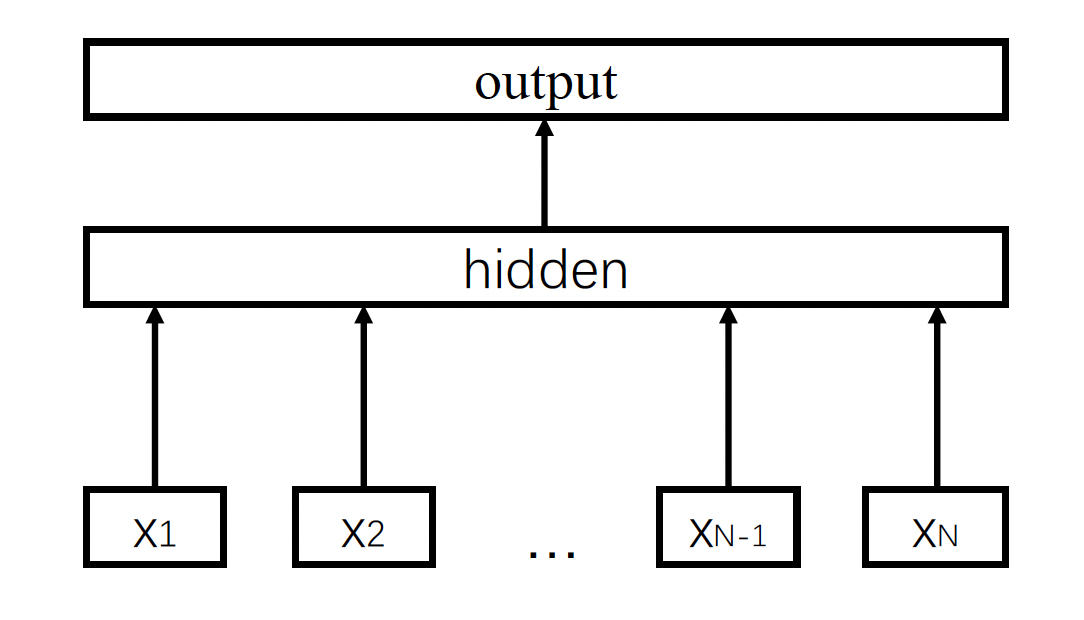
\includegraphics[width=0.9\textwidth]  {imgs/fasttext.png} \\
\bicaption[FastText \cite{joulin2016bag} 图示]
    {FastText \cite{joulin2016bag} 图示。}
    {Model architecure of FastText \cite{joulin2016bag}.}
\label{fig:fasttext}
\end{figure}

图\ref{fig:fasttext}为 FastText 的结构图。FastText 模型输入一个序列(可以是一句话,也可以是一段文本),输出这个序列在各个文本类别上的概率分布。FastText 模型结构和 Word2Vec 中的 CBOW 结构很相似,一共有三层,分别是输入层、隐藏层和输出层。首先将输入的序列划分为单词的特征向量,经过线性变换映射到隐藏层进行叠加求平均操作,最终线性变换映射到文本的类别标签。FastText 和 Word2Vec 的不同之处在于,在 Word2Vec 中将每一个单词视为要找到整个序列向量表示的最小单位;但在 FastText 中,采用 n-gram 对单词进行切分,即一个单词由 n-gram 个字符组成。为了加速训练的速度,FastText 中也采用了层级 softmax ,利用了类别分布不均衡的优势,通过使用哈夫曼编码建立基于类别表征的二叉树。因此,FastText 的核心工作是将构成序列的单词以及 n-gram 向量进行叠加平均操作得到序列向量,然后使用序列向量进行 softmax 多分类任务。

综上所述,FastText 使用一个浅层的神经网络能够达到媲美深度神经网络的分类精度,并且拥有高效的训练速度。可以在不使用 GPU 的情况下,利用 CPU 完成词嵌入向量的训练。Le 和 Huynh 等人\cite{le2019identifying} 结合 FastText 架构和氨基酸的嵌入表征来识别 SNARE。他们任务可以将 FastText 模型应用于生物信息学,可以为蛋白质测序预测提供基础。本文基于 FastText 模型结构构建了一个分类模型,可以同时用于蛋白质序列的嵌入表征学习以及蛋白质序列的分类任务。

\subsection{Doc2Vec}
Le 和 Mikolov 等人于 2014 年提出的 Doc2Vec 模型 \cite{le2014distributed} 是对 Word2Vec 模型的扩展。虽然 Word2Vec 可以提高比较准确的词向量,在一些任务中表现优异,但是还不存在一个有效的模型将它们结合成一个序列或者文档向量,因此 Doc2Vec 主要是对较大的文本块(例如段落或者整个文档等)的连续嵌入表示进行无监督学习。

和 Word2Vec 相似,Doc2Vec 也包含两个学习模型,一种是分布记忆的段落向量(PV-DM),类似于 Word2Vec 中的 CBOW 模型;另一种是分布词袋的段落向量(PV-DBOW),类似于 Word2Vec 中的 skip-gram 模型。
Doc2Vec 的训练过程和 Word2Vec 基本一致,每次迭代从一段话中利用滑动窗口采样固定长度的单词序列,其中的一个单词作为输出的预测词,其他单词作为输入词。不同之处在于,Doc2Vec 在 Word2Vec 的基础上增加了句子向量,同词向量一起作为输入层的输入,之后将所有的向量叠加求平均生成一个新的隐藏向量,进而使用这个隐藏向量预测滑动窗口内的预测词。句子向量在同一段文本的若干次滑动窗口迭代训练中是共享的,可以看作是该句子的主旨,因此拥有记忆功能,弥补了 Word2Vec 中忽略了本次窗口中训练的词以外文本中的其他词的不足。

Yang \cite{yang2018learned} 等人利用 Word2Vec 和 Doc2Vec 两种模型学习蛋白质的嵌入表征,由于蛋白质序列的长度相比普通的文本句子要长很多,因此 Doc2Vec 非常适合大文本的蛋白质序列嵌入表征学习。本文利用了 Doc2Vec 的 PV-DM 模型作为预训练任务学习蛋白质序列的嵌入表征。

\section{本章总结}
本章主要对本文中使用的当下流行的词嵌入方法进行了总结。我们按照词嵌入表征学习的研究历程介绍了三种词嵌入方法,包括基于离散表示的词嵌入方法,基于 SVD 分解的词嵌入方法,基于神经网络的词嵌入方法,其中基于神经网络的词嵌入方法是目前学界主流的表征学习方法。我们讨论了四种基于神经网络的词嵌入方法,包括 Word2Vec、GloVe、FastText 和 Doc2Vec,分别介绍了它们的实现方式以及目前在蛋白质序列表示学习中的研究成果。



